\documentclass{scrartcl}

\usepackage{siunitx, geometry, amsmath, amssymb, graphicx, subfig}

\title{Fundamentals of Simulation Methods}
\subtitle{Exercise 5}
\author{Patrick Schygulla}
\date{\today}


\begin{document}
\maketitle

\section*{5.1. FFT based convolution}
\paragraph*{(a)} We integrate over the entire plane to obtain the normalisation factor using the coordinate transformation $u = r/h$. There is no dependence on an angle so in polar coordinates the angular integral can be carried out immediately ($\int\mathrm{d}\phi = 2\pi$):
\begin{equation*}
	\begin{array}{rrcl}
	&	1 & = & \int\limits_{\mathbb{R}^2} W(|\vec{r}|)\mathrm{d}^2r \\
	&	  & = & 2\pi h^2 k \left( \int\limits_0^{1/2}\mathrm{d}u u(1-6u^2+6u^3) + \int\limits_{1/2}^1\mathrm{d}u u2(1-u)^3 \right) \\
	&	  & = & 2\pi h^2 k \; 0.0875 \\
	\Rightarrow & k & = & \frac{11.43}{2\pi h^2} \approx 1.819/h^2
	\end{array}
\end{equation*}

\paragraph*{(b) and (c)} The sum of all colour channels (red, green, blue) and of all pixels before and after smoothing differ by 241 which corresponds to a relative error of 4~ppm. The integral over the kernel differs from the desired value of 1 by \SI{4e-6}{} (cf. table~\ref{tab:check}). This difference could be further reduced by choosing a higher precision for the kernel, for instance long double, and defining the normalisation $k$ with more significant digits (here 14 digits were used). The images before and after smoothing can be found in fig.~\ref{fig:images}.
\begin{table}
	\centering
	\begin{tabular}{l|l}
		\textbf{before smoothing} & 62265510.0 \\
		\textbf{after smoothing}  & 62265269.9 \\
		\textbf{kernel integral}  & 0.999996144309 
	\end{tabular}
	\caption{Results of checking the consistency of the smoothing procedure.}
	\label{tab:check}
\end{table}
\begin{figure}
	\subfloat[Original image.]{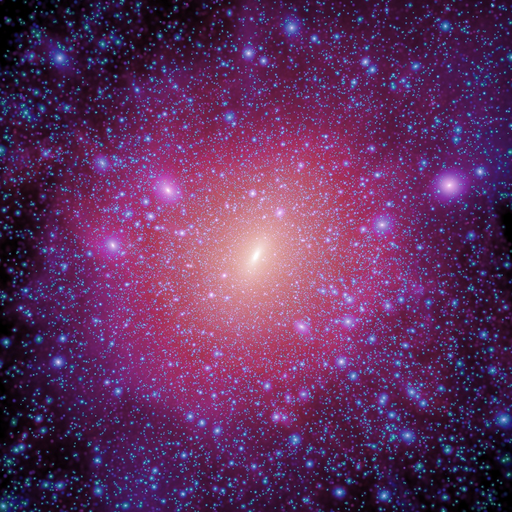
\includegraphics[width=0.45\textwidth]{aq-original.png}} \hfill
	\subfloat[Smoothed image.]{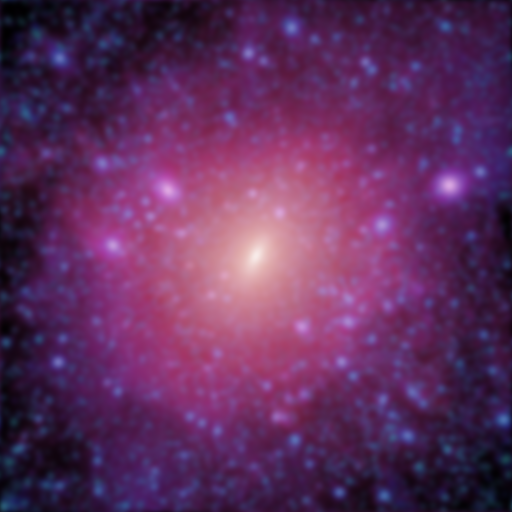
\includegraphics[width=0.45\textwidth]{aq-smoothed.png}}
	\caption{Comparison of original and smoothed image.}
		\label{fig:images}
\end{figure}

\end{document}